\begin{figure}[t]
    \centering
    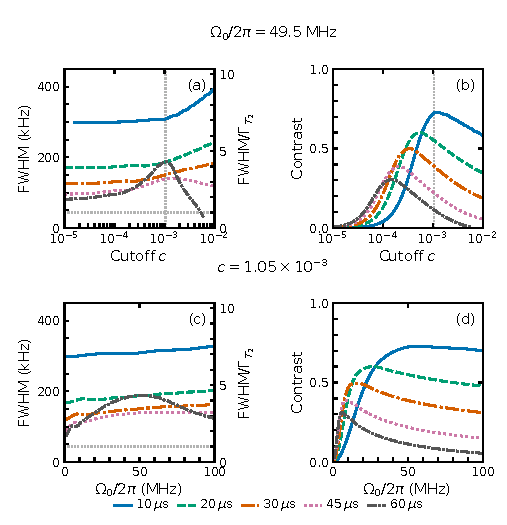
\includegraphics[width=\columnwidth]{../figures/paper/04_duration_cutoff_scan.pdf}
    \caption{Simulated cutoff and duration dependence of the polynomial-corrected DRAG echo.
    (a),(b) Normalized dip FWHM and contrast $C$ versus cutoff and drive
    amplitude for $L=30~\mu\mathrm{s}$.
    The white contours enclose the $C>0.2$ band, where panel (a) also
    shows narrow dips. Cutoff controls the pulse-core width; this band
    balances spectral narrowing against loss of contrast, retaining a
    distinguishable resonance over a broad amplitude range.
    (c),(d) Cutoff slices at $\Omega_0/(2\pi)=49.5~\mathrm{MHz}$
    (orange dashed lines) for durations $L=10$--$60~\mu\mathrm{s}$.
    The thick orange $30~\mu\mathrm{s}$ curves match the maps;
    dotted lines mark $\mathrm{FWHM}/\Gamma_{T_2}=1$ in (c) and $C=0.2$ in (d).}
    \label{fig:duration-cutoff-scan}
\end{figure}
